%!TEX root = ../report.tex
\section{Hardware Design Decisions}
\label{sec:hardware-decisions}
This section defines decisions made regarding the hardware selection. Tables will be used to make our justification in regard to hardware selection more crystal clear.

% ng180levee
\begin{table}[H]
	\begin{tabular}{L{0.2\textwidth} L{0.6\textwidth}}
		\textbf{Name}           & \textbf{Choice of dike sensor} \\ \toprule
		\textbf{Decision}       & \textbf{\req{hw}}\\ \midrule
		\textbf{Status}         & \textbf{Approved} \\ \midrule
		\textbf{Problem/Issue}  & The system needs a reliable sensor system to measure condition of dikes. \\ \midrule
		\textbf{Decision}       & The system will implement GeoBeads MEMS Sensor in dikes.\\ \midrule
		\textbf{Alternatives}   & \textit{GeoBeads}\\
		& The GeoBead is a compact sensor, which can measure the pore pressure, temperature and local tilt in dikes. A unit costs about 350 dollar\cite{ng180levee}. \\
		& \textit{Piezometers}\\
		& Piezometers measure the pore water pressure in the dikes. This information can be used to measure the stability of the dike. A piezometer costs about 200 dollar\cite{ng180levee}. \\
		& \textit{Volt meters} \\
		& Volt meters can be used to measure the streaming potential in the dike, which are an indicator of its stability\cite{selfpotential}. These sensors are approximately 50 dollars per unit. Materials in the dike can decrease the accuracy of this measurement technique. \\
		\midrule
		\textbf{Arguments}      & \\
		&   \begin{tabular}{l|lllllll|l}
		& \rot{Reliability} & \rot{Resilience} & \rot{Performance} & \rot{Interoperability} & \rot{Security} & \rot{Scalability} & \rot{Cost} & \rot{\textbf{Score}} \\ \hline
		%                rel res per int sec sca cost
		Weights        	& 3 & 2 & 3 & 2 & 2 & 2 & 2 \\ \hline
		GeoBeads        & 5 & 4 & 4 & 2 & 2 & 3 & 2 & 53 \\ 
		Piezometer      & 4 & 2 & 3 & 2 & 2 & 3 & 3 & 45 \\
		Volt meters 	& 1 & 5 & 3 & 2 & 2 & 3 & 5 & 46 \\
	\end{tabular} \\
	\\ \bottomrule
	\end{tabular}
	\caption{Decision -- Choice of Sensors}
	\label{table:linux}
\end{table}


% ng180levee
\begin{table}[H]
	\begin{tabular}{L{0.2\textwidth} L{0.6\textwidth}}
		\textbf{Name}           & \textbf{Connectivity of the dike sensor} \\ \toprule
		\textbf{Decision}       & \textbf{\req{hw}}\\ \midrule
		\textbf{Status}         & \textbf{Approved} \\ \midrule
		\textbf{Problem/Issue}  & The dike sensors have to be connected to the internet in some way, so they can send their data to the central server. \\ \midrule
		\textbf{Decision}       & The sensors will be connected by a wire.\\ \midrule
		\textbf{Alternatives}   & \textit{Wired}\\
		& A wired cable connects the dike sensor. This cable can also be used to supply the sensor with electricity. \\
		& \textit{ZigBee}\\
		& ZigBee is an open protocol for personal area networks. It uses little power and is therefore a good choice for devices equipped with a battery. \\
		& \textit{ISM radio band} \\
		& The ISM radio bands can be used for industrial, scientific and medical purposes.  \\
		\midrule
		\textbf{Arguments}      & ZigBee is not an option, since the sensors are embedded in the soil of the dikes, and the frequency it uses, decreases too much in strength when traveling through the dike\cite{van2009draadloos}. \\
		& Research has been done by van der Gees and Kok \cite{van2009draadloos} to determine if it is feasible to use the ISM radio band to communicate from within the dike. They concluded that, while it is possible to communicate through the dike using this band, the distance is limited and the rate of error is relatively high.
		\\
		& While a wire is not ideal in the sense that it will have to connect all the sensors, it seems to be the best option for the sensor in the dikes. It has the additional benefit that it can also supply the sensors with electricity.
						                            
		\begin{tabular}{l|lllllll|l}
		               & \rot{Reliability} & \rot{Resilience} & \rot{Performance} & \rot{Interoperability} & \rot{Security} & \rot{Scalability} & \rot{Cost} & \rot{\textbf{Score}} \\ \hline
		%               rel res per int sec sca cost
		Weights        & 3 & 2 & 3 & 2 & 2 & 2 & 2 \\ \hline
		Wired          & 5 & 4 & 3 & 3 & 2 & 2 & 2 & 50 \\ 
		ZigBee         & 4 & 2 & 2 & 2 & 2 & 4 & 3 & 42 \\
		ISM Radio band & 1 & 5 & 2 & 2 & 2 & 3 & 5 & 43 \\
	\end{tabular} \\
	\\ \bottomrule
	\end{tabular}
	\caption{Decision -- Connectivity of the dike sensor}
	\label{table:linux}
\end{table}

\begin{table}[H]
	\begin{tabular}{L{0.2\textwidth} L{0.6\textwidth}}
		\textbf{Name}           & \textbf{Data Gathering from Sensors} \\ \toprule
		\textbf{Decision}       & \textbf{\req{hw}}\\ \midrule
		\textbf{Status}         & \textbf{Approved} \\ \midrule
		\textbf{Problem/Issue}  & There must be single board computer that handles connection from sensors to Data Collecting System. \\ \midrule
		\textbf{Decision}       & Arduino Uno Ethernet will bridge between sensors and Data Collecting System.\\ \midrule
		\textbf{Alternatives}   & \textit{Arduino Uno}\\
		& A low cost but powerful single board computer that can be programmed as needed. Arduino Uno has high extendability because it can be equipped with Arduino shield that will expand its capabilities. The minus point of this type is it does not have built in Ethernet jack. \\
		& \textit{Arduino Uno Ethernet}\\
		& This is basically the same as Arduino Uno. However, it has built in Ethernet jack.\\
		& \textit{Arduino Mega}\\
		& This type of Arduino has more flash storage and SRAM. However, the physical size of this device is also significantly bigger.\\
		\midrule
		\textbf{Arguments}      & The most suitable Arduino for the SMF is the Arduino Uno Ehternet because it has built-in Ethernet jack. Thus, the remaining expansion port will remain free for future evolution purpose. This way, the energy consumption of Arduino will also be low because it does not have any extension shield. We assume that Arduino will be powered by power landline connection of telecom provider.
						
		\begin{tabular}{l|lllllll|l}
		                     & \rot{Reliability} & \rot{Resilience} & \rot{Performance} & \rot{Interoperability} & \rot{Security} & \rot{Scalability} & \rot{Cost} & \rot{\textbf{Score}} \\ \hline
		%                             rel res per int sec sca cost
		Weights              & 3 & 2 & 3 & 2 & 2 & 2 & 2 \\ \hline
		Arduino Uno          & 4                 & 3                & 3                 & 3                      & 2              & 3                 & 5          & 53                   \\ 
		Arduino Uno Ethernet & 4                 & 3                & 3                 & 5                      & 2              & 3                 & 4          & 55                   \\
		Arduino Mega         & 4                 & 3                & 3                 & 3                      & 2              & 3                 & 3          & 49                   \\
	\end{tabular} \\                 
			
	\\ \bottomrule
	\end{tabular}
	\caption{Decision -- Arduino selection}
	\label{table:linux}
\end{table}

%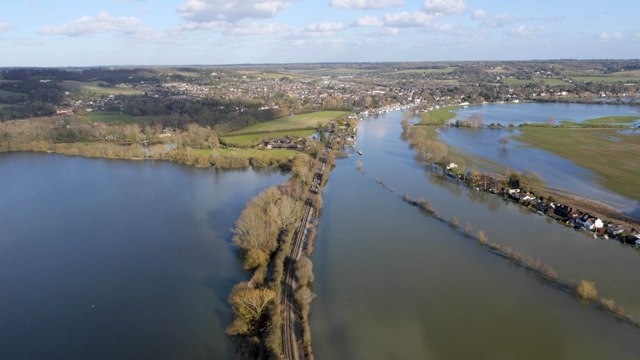
\includegraphics[scale=0.5]{6-hardware/images/uavflood.jpg}
\begin{table}[H]
	\begin{tabular}{L{0.2\textwidth} L{0.6\textwidth}}
						
		\textbf{Name}          & \textbf{UAVs}                                                                                                                                                              \\ \toprule
		\textbf{Decision}      & \textbf{\req{hw}}                                                                                                                                                             
								\textit{A2 Multi spectral X4} \\ 
								& Flight mode : GPS, computer based, Time of flight, long range:90 min. \\                                                                                        
								% Price : 9000
								%\textit{Skyjib 8 Titanium} \\ 
								%& Flight mode : GPS, computer based, Time of flight :  12-25 min  , Speed : 12m/s. \\                                                                                         \midrule
		\textbf{Status}        & \textbf{Approved}                                                                                                                                                          \\ \midrule
		\textbf{Problem/Issue} & The system uses UAV's in order to get more data during a flood and to create a map of the flooded area.                                                                    \\ \midrule
		\textbf{Alternatives} 
		                       & \textit {Skyjib Super 6 Ti-QR}                                                                                                                                             \\
		                       & Flight mode : GPS, computer based, Time of flight : 10 minutes , Speed : 10 m/s. Can only support GroPro.                                                                
		                       
		                       \\
		                       & \textit {DJI Phantom 3}                                                                                                                                                    \\
		                       & Flight mode : GPS, computer based, Time of flight : 15 minutes , Speed : 10 m/s.                                                                                          \\ 
		\midrule
		\textbf{Arguments}     & Getting high quality data quickly : photograph and 360 deg videos . Produce accurate and high resolution surveys .                                                         \\
		                       & Cost effective.                                                                                                                                                            \\ 
		                       & View to hard-to-reach and dangerous(where the man cannot go) areas which ensures safety because it does not require personnel to enter potentially hazardous environments. \\                          
		                       & Establishment of Elevation Models to assess water flow direction and accumulation.                                                                                       
		                       
		                       		\begin{tabular}{l|lllllll|l}
		                     & \rot{Reliability} & \rot{Resilience} & \rot{Performance} & \rot{Interoperability} & \rot{Security} & \rot{Scalability} & \rot{Cost} & \rot{\textbf{Score}} \\ \hline
		%                             rel res per int sec sca cost
		Weights               & 3 & 2 & 3 & 2 & 2 & 2 & 2 \\ \hline
		Skijib 8 Titanium         & 4                 & 3                & 4                 & 3                      & 3              & 3                 & 2          &   52            \\ 
		Skyjib Super 6 Ti-QR & 4                 & 3                & 3                 & 3                      & 2              & 3                 & 4          &   51                \\
		Dji Phantom 3         & 3                 & 3                & 3                 & 3                      & 2              & 3                 & 3          &    46               \\
	\end{tabular} \\   \\ 
						                           
						                               
						
		\\ \bottomrule
	\end{tabular}
	\caption{Decision -- UAVs}
	\label{table:linux}
\end{table}


\begin{table}[H]
	\begin{tabular}{L{0.2\textwidth} L{0.6\textwidth}}
		\textbf{Name}           & \textbf{Analytic cluster selection} \\ \toprule
		\textbf{Decision}       & \textbf{\req{hw}}\\ \midrule
		\textbf{Status}         & \textbf{Approved} \\ \midrule
		\textbf{Problem/Issue}  & SFM needs a reliable computers to do the analytical processing. \\ \midrule
		\textbf{Decision}       & SFM will use clustered Dell PowerEdge R530 to act as the main analytic cluster and to provide API to the actors.\\ \midrule
		\textbf{Alternatives}   & \textit{HP ProLiant DL360 Gen9 Base}\\
		% https://www.google.nl/shopping/product/12299869794181781707?biw=1346&bih=669&q=servers&bav=on.2,or.r_cp.&bvm=bv.104317490,d.d2s&ion=1&espv=2&tch=1&ech=1&psi=1FIQVpOAEoPlaK7Zn4AN.1443910356406.15#sgro=om
		& This server rack has 16GB of memory and 2.4GHz of processor speed. As other server computer, this machine utilizes Intel Xeon E5 2600v3. This server is suitable for high dense computing, however the price is not so suitable for this kind of specification. It does not have LCD screen that will help technician to look the current status of the server.\\
		& \textit{Lenovo System x3550 M4 7914}\\
		% https://www.google.nl/shopping/product/8704926690761174474?q=servers&biw=1346&bih=669&bav=on.2,or.r_cp.&bvm=bv.104317490,d.d2s&ion=1&espv=2&tch=1&ech=1&psi=1FIQVpOAEoPlaK7Zn4AN.1443910356406.17
		& This server rack has only 8GB of memory. However, the processor is a bit faster, it runs on 2.6GHz. As other server computer, this machine also utilizes Intel XEON E5-2600. The price is a little bit lower than the others but the memory limitation makes it not so valuable. It has LCD screen that will help technician to look the current status of the server. \\
		& \textit{Dell PowerEdge R530} \\
		% https://azerty.nl/0-3031-817940/dell-poweredge-r530-server-rack-uitvoering-2u-2-weg-1-x-xeon-e5-2620v3-2-4-ghz-ram-16-gb-sas-hot-swap-verwiss.html?channel_code=544&s2m_campaign=1CENT&s2m_product_id=817940
		& This 2U server rack has 16GB of memory and 2.4GHz of processor speed. This machine utilizes Intel Xeon E5-2620V3 with 15MB of cache. This server is suitable for high dense computing. It has LCD screen that will help technician to look the current status of the server. \\
		\midrule
		\textbf{Arguments}      & \\
		&   \begin{tabular}{l|llllll|l}
		                                  & \rot{Reliability} & \rot{Performance} & \rot{Interoperability} & \rot{Security} & \rot{Scalability} & \rot{Cost} & \rot{\textbf{Score}} \\ \hline
		%                                        rel res per int sec sca cost
		Weights                         3 & 2 & 3 & 2 & 2 & 2 & 2 \\ \hline
		Dell PowerEdge R530             5 & 3                 & 5                 & 4                      & 4              & 4                 & 5          & 70                   \\ 
		Lenovo System x3550 M4 7914     4 & 3                 & 4                 & 4                      & 3              & 4                 & 4          & 60                   \\
		HP ProLiant DL360 Gen9 Base     5 & 3                 & 5                 & 4                      & 3              & 4                 & 3          & 64                   \\
	\end{tabular} \\
	\\ \bottomrule
	\end{tabular}
	\caption{Decision -- Analytic cluster selection}
	\label{table:server-selection}
\end{table}

\begin{table}[H]
	\begin{tabular}{L{0.2\textwidth} L{0.6\textwidth}}
		\textbf{Name}           & \textbf{Database cluster selection} \\ \toprule
		\textbf{Decision}       & \textbf{\req{hw}} \\ \midrule
		\textbf{Status}         & \textbf{Approved} \\ \midrule
		\textbf{Problem/Issue}  & The system needs reliable computers to store the data. \\ \midrule
		\textbf{Decision}       & SFM will utilize Synology RackStation RS814RP to store the data.\\ \midrule
		\textbf{Alternatives}   & \textit{Synology RackStation RS814RP}\\
		% https://www.google.nl/shopping/product/9793555443596138172?biw=1346&bih=669&q=storage+servers&bav=on.2,or.r_cp.&bvm=bv.104317490,d.d2s&ion=1&espv=2&tch=1&ech=1&psi=1FIQVpOAEoPlaK7Zn4AN.1443910356406.23&prds=paur:ClkAsKraX8aViW9QBHq_YeLbadvaW6lnMVQDuwzotG6gRVknHILZ_EDzrO8nQNS6N477UjRspRo17BmUoyZnQjMDnOrhflRLM5VXFQCOPDxn9wCZnGJxrWXfWxIZAFPVH73DWMclCanKIzQ68mJVd6ADLpvTfg&sa=X&ved=0CMkDEM1KMBJqFQoTCLid3qaqp8gCFYrZGgodX70Kow
		& This storage machine has the fastest connection among the others. This machine will run at SATA with 6 Gbps connection.\\
		& \textit{70BJ NAS-server}\\
		% https://www.google.nl/shopping/product/15463250681911940369?q=storage+servers&biw=1346&bih=669&bav=on.2,or.r_cp.&bvm=bv.104317490,d.d2s&ion=1&espv=2&tch=1&ech=1&psi=1FIQVpOAEoPlaK7Zn4AN.1443910356406.25&prds=paur:ClkAsKraXy1_BVqi5aD5CGi7OmupTi3OwyL-j7nW7Ss2Qwo-W_81sjaidQU8J0Q3uu7RrSCCth3c9YuMEMNA3zO6TM9tfutSn6ksUeo1EGFdUDKUIlB4gt8wBBIZAFPVH70byN_Dqe5qhSCABb7sxVXYXAvfaw&sa=X&ved=0CIEDEM1KMAo4FGoVChMIpJb_tKqnyAIVQUwaCh0d6wGT
		& This machine form factor is 1U which is suitable for saving space. However, the connection speed is limited to 3 Gbps.\\
		& \textit{Thecus N8810U-G NAS-server} \\
		% https://www.google.nl/shopping/product/464537487289413504?q=storage+servers&biw=1346&bih=669&bav=on.2,or.r_cp.&bvm=bv.104317490,d.d2s&ion=1&espv=2&tch=1&ech=1&psi=1FIQVpOAEoPlaK7Zn4AN.1443910356406.25&prds=paur:ClkAsKraXylXtQJRG2pDp_XW-OBbRHsXe6nrmcB3olgeJQi1FhG4T8bXQABWVbkevi6hzBMwfTk7qioWd88Cq3GWIt3hQlEi5oJEmR7vZvXtvtEinYYlhn3_bBIZAFPVH71qflxmS1BuYghV4B5tpcohhFU7vQ&sa=X&ved=0CNQCEM1KMAU4FGoVChMIpJb_tKqnyAIVQUwaCh0d6wGT
		& This machine also runs in 3Gbps connection. However, the form factor is 2U which makes this machine takes more space in the rack.\\
		\midrule
		\textbf{Arguments}      & \\
		&   \begin{tabular}{l|llllll|l}
		                                  & \rot{Reliability} & \rot{Performance} & \rot{Interoperability} & \rot{Security} & \rot{Scalability} & \rot{Cost} & \rot{\textbf{Score}} \\ \hline
		%                                rel res per int sec sca cost
		Weights                         3 & 2 & 3 & 2 & 2 & 2 & 2 \\ \hline
		Synology RackStation RS814RP    5 & 2                 & 4                 & 4                      & 4              & 4                 & 4          & 63                   \\ 
		70BJ NAS-server                 4 & 2                 & 3                 & 4                      & 4              & 4                 & 3          & 55                   \\
		Thecus N8810U-G NAS-server      4 & 2                 & 3                 & 4                      & 4              & 4                 & 3          & 55                   \\
	\end{tabular} \\
	\\ \bottomrule
	\end{tabular}
	\caption{Decision -- Choice of storage machine.}
	\label{table:database-selection}
\end{table}

\begin{table}[H]
	\begin{tabular}{L{0.2\textwidth} L{0.6\textwidth}}
		\textbf{Name}           & \textbf{High Performance Switch selection} \\ \toprule
		\textbf{Decision}       & \textbf{\req{hw}}\\ \midrule
		\textbf{Status}         & \textbf{Approved} \\ \midrule
		\textbf{Problem/Issue}  & SFM cluster needs a powerful high performance switch to connect each cluster. \\ \midrule
		\textbf{Decision}       & SFM will use Cisco Catalyst 2960S-24TS-L Switch.\\ \midrule
		\textbf{Alternatives}   & \textit{Linksys LGS552P Switch}\\
		% https://www.google.nl/shopping/product/15955701749855379542?biw=1346&bih=669&q=network+switch&sqi=2&bav=on.2,or.r_cp.&bvm=bv.104317490,d.d2s&ion=1&espv=2&tch=1&ech=1&psi=1FIQVpOAEoPlaK7Zn4AN.1443910356406.33&prds=paur:ClkAsKraX5ryPFpohZJ3cHRR5Y04pVrqqvR-5nXru2N7X2-97H3V7DAZtCjwWh2BPthulxNJ2ahSWe7PR9qBPpG4AcckL_q3UHXeyd1fqIcsRCo9aEhM_4ihYhIZAFPVH7186CU9loBEx5Tx9iwfjvLu2xB6eg&sa=X&ved=0CM4CEM1KMAJqFQoTCJaXr-ahqMgCFUh-Ggodym4G5w
		& This switch has 52 ports available for connection, which is very good for scalability. However the performance is not as good as Cisco catalyst switch series.\\
		& \textit{HP 1820-48G Switch}\\
		% https://www.google.nl/shopping/product/7539423950361123669?biw=1346&bih=669&q=network+switch&sqi=2&bav=on.2,or.r_cp.&bvm=bv.104317490,d.d2s&ion=1&espv=2&tch=1&ech=1&psi=1FIQVpOAEoPlaK7Zn4AN.1443910356406.33&prds=paur:ClkAsKraX2rp4gF8ATRwWJuY5iaZuchaa1sdhIz6lvepgxugqRb5mZxy8yAXts_70QyVg33fwd3C8WiFm3ThxDkZDi6gz2-ogcVLZ1Frs8QHH9IhEd-rj9s-CBIZAFPVH71WuYA_yyIRCl_FpDi93AJr9DX5QQ&sa=X&ved=0CNgCEM1KMANqFQoTCJaXr-ahqMgCFUh-Ggodym4G5w
		& This switch has lesser available ports than Linksys switch. It has 48 ports available. This switch is not very configurable which makes this not so suitable for high performance switching. \\
		& \textit{Cisco Catalyst 2960S-24TS-L Switch} \\
		% https://www.google.nl/shopping/product/3278668597556943908?biw=1346&bih=669&q=network+switch&sqi=2&bav=on.2,or.r_cp.&bvm=bv.104317490,d.d2s&ion=1&espv=2&tch=1&ech=1&psi=1FIQVpOAEoPlaK7Zn4AN.1443910356406.33&prds=paur:ClkAsKraXw_7YyEqvAKzRJjfEM3yN-4kzC4NaE-smcis8WFMegcToXlCuBmXRPb647qqqZU34GfFxp8EYHh7FC1AVCwaCRNTWcvFYI4Ppe8B8xT_2AMPJ7r3XBIZAFPVH72nlGbb8LwIOpZWGX8ZHfTvUUmDSw&sa=X&ved=0CPUCEM1KMAZqFQoTCJaXr-ahqMgCFUh-Ggodym4G5w
		& This switch has the lowest number of port available, 24 ports. However, Cisco Catalyst is very configurable and has a very good security. \\
		\midrule
		\textbf{Arguments}      & \\
		&   \begin{tabular}{l|llllll|l}
		                                      & \rot{Reliability} & \rot{Performance} & \rot{Interoperability} & \rot{Security} & \rot{Scalability} & \rot{Cost} & \rot{\textbf{Score}} \\ \hline
		%                                    rel res per int sec sca cost
		Weights                             3 & 2 & 3 & 2 & 2 & 2 & 2 \\ \hline
		Cisco Catalyst 2960S-24TS-L Switch  5 & 2                 & 5                 & 4                      & 5              & 3                 & 4          & 66                   \\ 
		Linksys LGS552P Switch              4 & 2                 & 4                 & 4                      & 3              & 4                 & 5          & 60                   \\
		HP 1820-48G Switch                  3 & 2                 & 4                 & 4                      & 3              & 4                 & 5          & 57                   \\
	\end{tabular} \\
	\\ \bottomrule
	\end{tabular}
	\caption{Decision -- Choice of high performance switch}
	\label{table:switch-selection}
\end{table}